\section{Science Data Quality Assurance}
\label{sec:sdqa}

\subsection{Overview of SDQA}

Science Data Quality Assurance (SDQA) describes a collection of
capabilities for Quality Analysis (QA) and Quality Control (QC) that
collectively ensure a high quality performing software system as well
as the ability to meet the scientific goals of the system. These are
designed to service LSST's quality assessment needs through all phases
of Construction, Commissioning and Operations. Consumers of these
services may include developers, facility staff, DAC (e.g., Level 3)
users, and the general LSST science user community.

SDQA capabilities can be divided into Quality Analysis (QA) and
Quality Control (QC) Capabilities.

\subsubsection{Quality Analysis (QA)}

Quality Analysis describes a range of \emph{activities} aimed at understanding the algorithmic performance of the code and eventually the properties of the data. These are achieved by a set of \emph{tools} that leverage components of the Data Management subsystem, as well as additional capabilities as necessary, to allow for the scientific inspection of data both by DM developers and scientists during construction as well as commissioning engineers and scientists during commissioning and operations.

QA activities include processing, analysing and inspecting data for forensic purposes. They also include the development of tests for verifying and characterising algorithmic performance, and are closely tied to the development of the Science Pipelines and the Science User Interface.

\subsubsection{Quality Control (QC)}

Quality Control describes a range of \emph{services and processes} aimed at measuring and monitoring and characterising the system (both software and data) to verify and characterise its performance. Whereas Quality Assurance describes the activities of people, Quality Control describes systems running autonomously and only notify people when an anomaly that cannot be automatically rectified is detected.

QC services include regression detection, measurement of Key Performance Metrics, a notification infrastructure and quality monitor dashboards. They are primarily the responsibility of the Science Quality and Reliability Engineering (SQuaRE) team.

\subsection{Key Features of SDQA (QA and QC) systems}

\begin{itemize}
\item SDQA provides capabilities for science data quality analysis of Level 1, 2, and Calibration Processing pipelines.

\item SDQA provides services to support software development in Construction, Commissioning and Operations.

\item SDQA provides for the visualization, analysis and monitoring capabilities needed for common science quality data analysis use cases. Its inputs may be gathered from SDQA services, the production pipelines, engineering data sources and non-LSST data sources.

\item SDQA has the flexibility to support execution of ad-hoc (user-driven) tests and analyses of ad-hoc datasets (provided they are supported by the LSST stack) within a standard framework.

\item SDQA supports use cases involving interactive ``drill-down'' of QC data exposed through its visualization interfaces.

\item SDQA allows for notifications to be issued when monitoring quantities that fall outside permissible bounds and/or have degraded over historical values.

\item SDQA is able to collect and harvest the outputs and logs of execution of a pipeline, and extract and expose metrics from these logs.

\item SQDA makes provision to store outputs that are not stored through other LSST data access services.

\item SDQA is deployable as high-reliability scalable services for production as well as allow for core data assessment functionality to be executed on a developer's local machine.

\item SDQA is architected in a manner that would enable it to be deployable on standard cloud architectures outside of the LSST facilities so that community-based L3 development activities can be supported.

\end{itemize}

\subsection{Key Tasks for Each Tier of QC}

SDQA system provides a framework that is capable of monitoring QC information at four different stages of capability and maturity:

\begin{itemize}
\item[QC Tier 0] Testing and Validation of the DM sub-system during software development
\item[QC Tier 1] Real-time data quality and system assesment during commissioning and operations (also, forensics)
\item[QC Tier 2] Quality assessment of Data Releases (also, forensics)
\item[QC Tier 3] Ability for the community to evaluate the data quality of their own analyses. These should made available as well-documented and deployable versions of core QC Tier 0--2 services.
\end{itemize}

A view of the tiered QC services is shown in \ref{fig:qa-overview}. Capabilities are increasingly layered (eg. tier QC-1 includes QC-0 services). A definition of the QC tiers is given in the rest of this section.

\begin{figure}
\centering
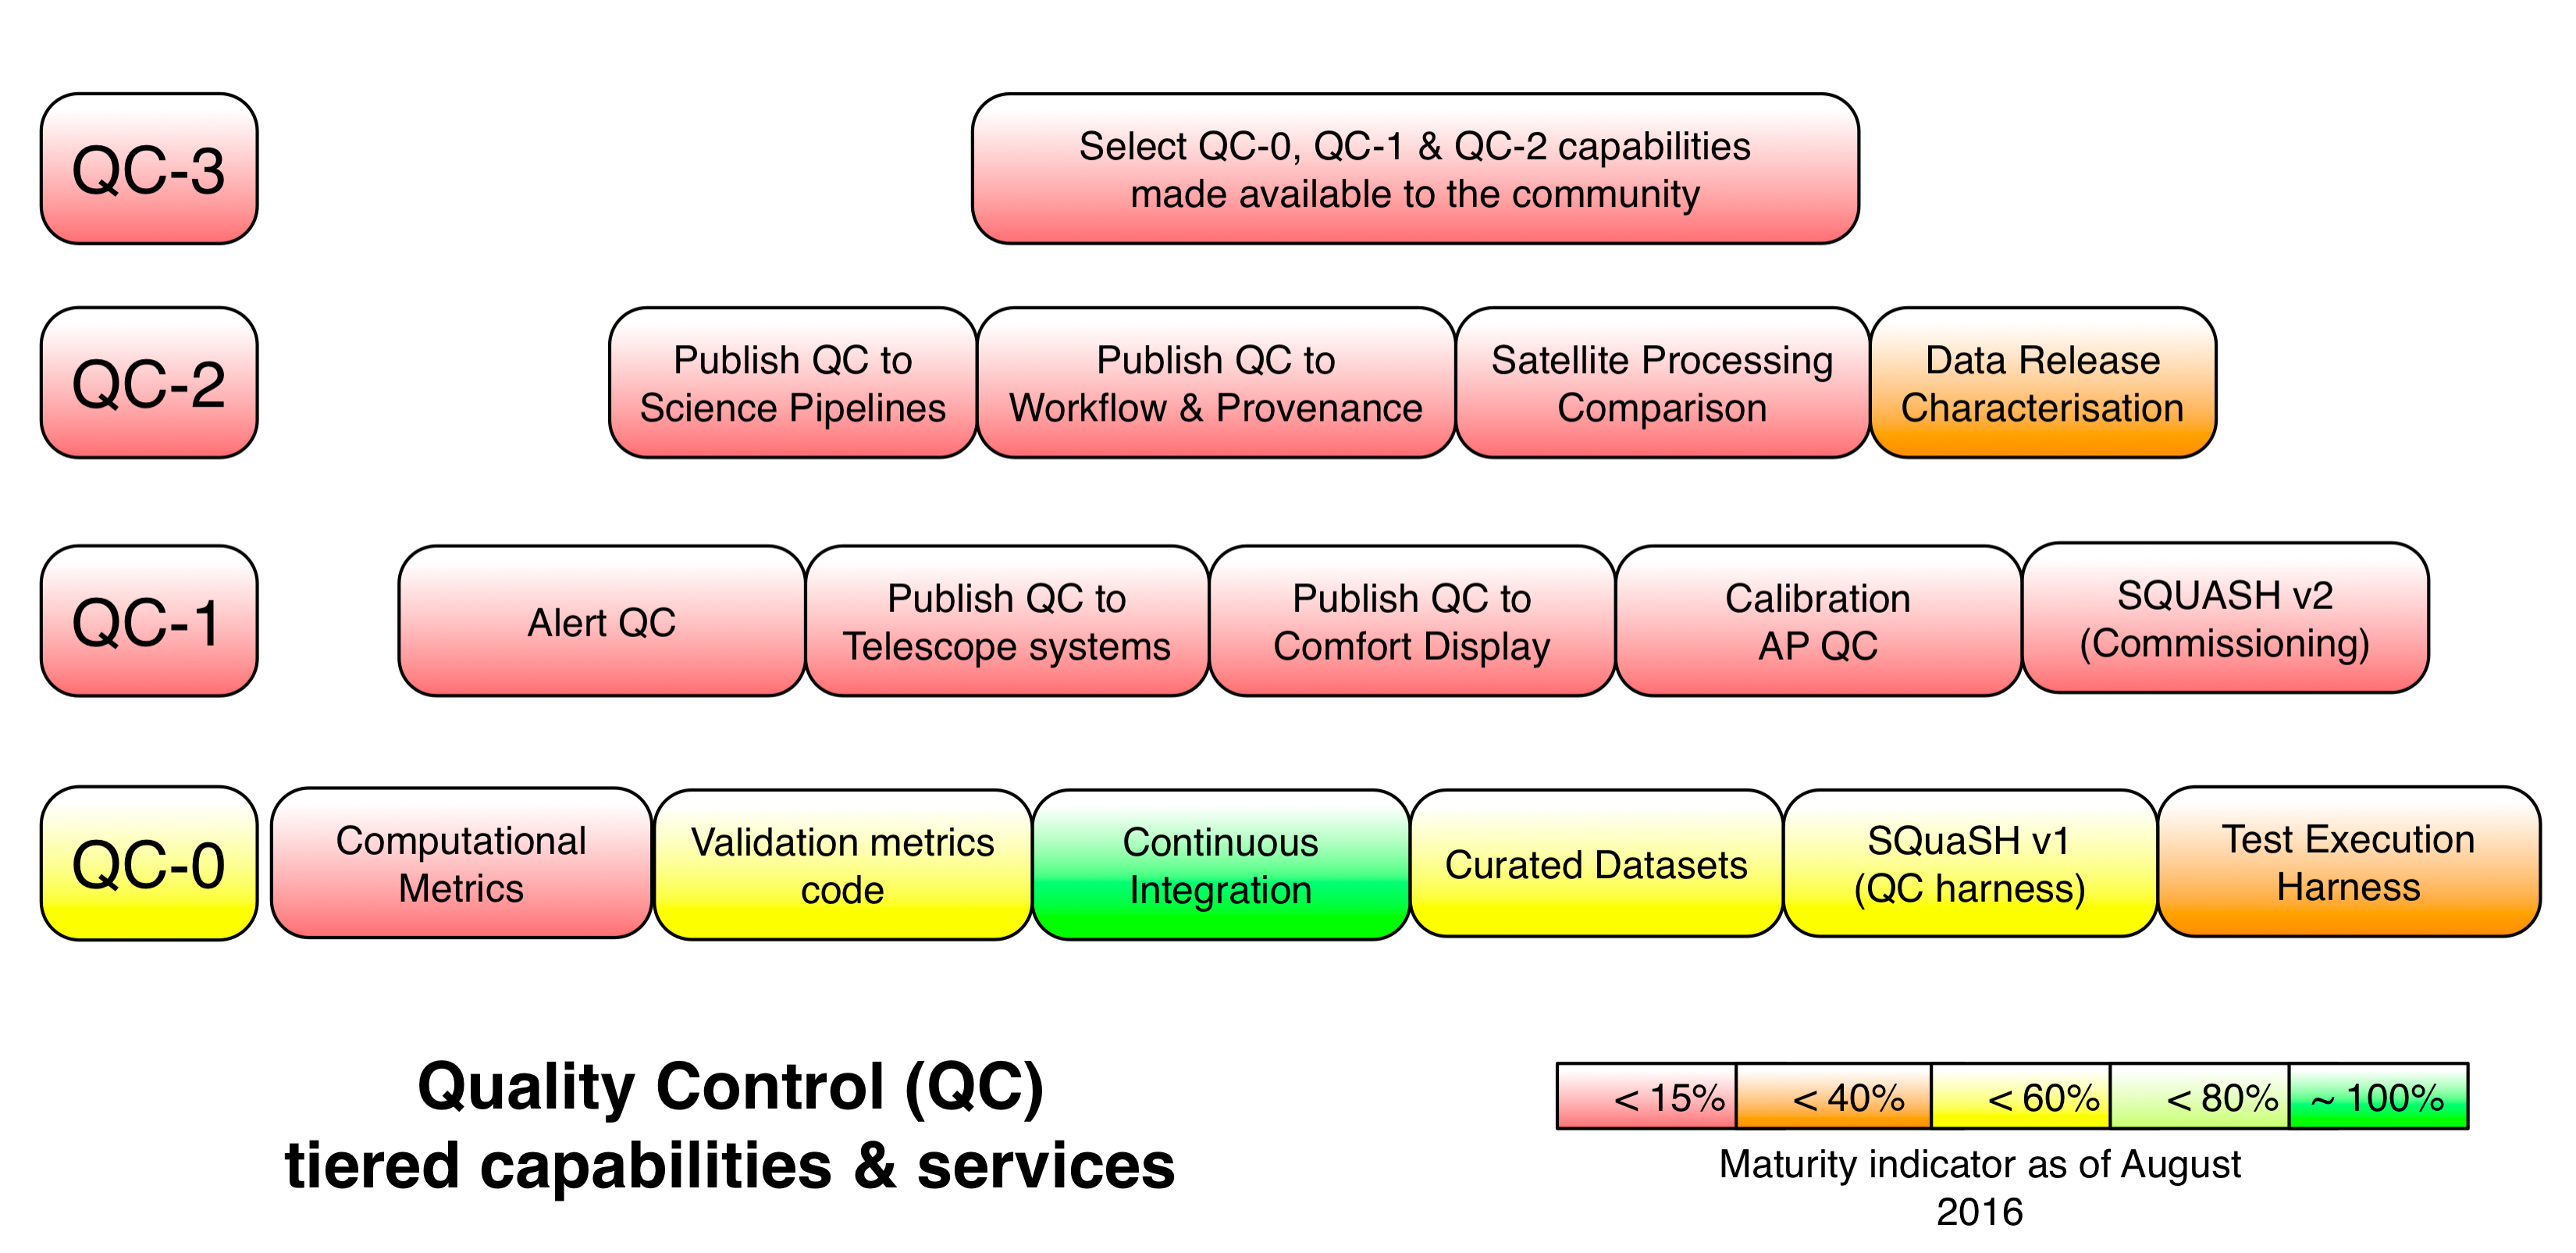
\includegraphics[width=\textwidth]{figures/qa_services.png}
\caption{Layer of progressive QC capabilities across all 4 tiers of QC.
\label{fig:qa-overview}}
\end{figure}



\subsubsection{QC Tier 0}

The first step to good quality data is good quality software. The purpose of QC-0 services is to enable testing of the DM software during development as well as validate software improvements during commissioning and operations, quantifying the software performance against known and/or expected inputs and outputs.

The core capabilities of QC-0 services are:

\paragraph{Continuous Integration Services}
\label{sec:qaCI}
\begin{itemize}

\item Continuous integration services compile code to uncover build errors and to trap failures in unit tests.

\item Builds of references (tags, branches) that can happen on a schedule, on developer request or on development events (e.g.,  merge to master)

\item SDQA provides CI services on multiple reference platforms and uses OS and compiler portability testing as a way to ensure the codebase is well engineered for future use.

\end{itemize}

\paragraph{Test Execution Harness}
\label{sec:qaTestharness}
\begin{itemize}

\item A test execution harness runs tests (such as data analysis unit
  tests) on a regular cadence (e.g.\ nightly/weekly/monthly) to allow
  basic functional checkout of the code. Tests written as part of Tier
  1-3 QC can be added directly by developers and be caused to execute
  without manual intervention, for example by checking in code or a
  specification in a purpose built test repository.

\item The test execution harness also allows the selection of a number of appropriate reference datasets (see \ref{sec:qaCurateddata}

\item Results from such tests are exposed in such a way as to allow summary reports and meaningful failure notifications.

\end{itemize}

\paragraph{Verification Metrics Code}
\label{sec:qaVerify}
\begin{itemize}

\item During Construction, progress towards meeting DM subsystem requirements revolve around the Key Performance Metrics (KPMs) outlined in LDM-240. SDQA implements code to calculate these KPMs. Consult \emph{reference to KPM Verification document} for a list of those metrics and how (and by whom and on what) they will be calculated.

\item Additional metrics must be calculated to be met in order for the DM subsystem to demonstrate its operational readiness. The list of those metrics and how (and by whom) they will be calculated will be in \emph{reference to DM Verification Plan CoDR document}. In terms of QC infrastructure, these metrics will not require different capabilities than the KPMs.

\item Verification code will be implemented in such a way that it can run with normal pipeline processing on developer's laptops, either inline or as after-burners as appropriate.

\item Additional metrics may be proposed during construction that are helpful to development or algorithm characterisation, either by developers investigating algorithms or as part of characterising the complete scientific and computational performance of the DM subsystem. SDQA will provide ways of executing that code in a similar way to KPMs, but apps developers may need to contribute the code (or at least document the algorithmic approach) to calculate those metrics.

\end{itemize}

\paragraph{Computational Metrics}
\label{sec:qaComputational}
\begin{itemize}

\item While the scope of this document is the scientific aspects of the pipelines, SDQA must also accommodate non-scientific KPMs and other metrics, such as computational performance characterisation.

\item SDQA will provide a capability to instrument the production pipelines to calculate computational performance metrics, and harvest data from those instrumentations (via logs or more direct ways of populating the QC database tables).

\item The computational performance metrics that SDQA calculates will be in practice surrogates for the actual computational performance in production since those will depend on the production system architecture. The purpose of calculating those as part of SDQA is to continuously monitor relative performance to alert the developers that a regression has occurred.

\item SDQA can calculate modeled system performance from the surrogate computational metrics if a model is provided to it (e.g., from Architecture).

\item A library of these instrumentations will be provided so that they can be mixed and matched to pipelines depending on the performance metric of interest.

\end{itemize}

\paragraph{Curated Datasets}
\label{sec:qaCurateddata}
\begin{itemize}

\item Part of the process for validating the software and its performance is selecting rich but targeted standardized data sets to generate directly comparable metrics between different versions of the software.

\item SDQA will select and curate a combination of simulated and precursor datasets that are modest enough for ``canary'' test runs but rich enough to characterise the envelope of algorithmic performance.

\item SDQA will ``publish'' (make available) these datasets so developers can run the validation tests directly against them in their own environments.

\end{itemize}


\paragraph{SQUASH - Science Quality Analysis Harness}
\label{sec:qaSquash}

SQUASH is a QC-as-a-service architecture that comprises the following elements:

\begin{enumerate}

\item The execution of simple pipeline workflows for the purposes of QC

\item The construction of those QC workflows with an emphasis on usability (not necessarily performance)

\item The collection and exposure of the results of those runs for further retrieval and analysis

\item A monitoring system to detect threshold trespass and excursions from past trends

\end{enumerate}

Notes:

\begin{itemize}

\item As construction progresses, first-party DM systems to underwrite the functions of SQUASH will become production ready. In the meantime, basic implementations of minimum viable functionality may be done with boostrap or off-the-shelf solutions either as an interim measure or, in some cases, a more lightweight solution (for example, working around features the butler does not have yet).

\item A simple example of a ``factory'' analysis based on SQUASH is ``Calculate the astrometric repeatability on this dataset; display the trend; drill down to to show the histogram of the points that went into calculating this trend''.

\item An advanced example of a bespoke analysis based on SQUASH is ``Display a three-color diagram of the sources in this run; compute the width of point sources in the selected -- e.g., blue -- part of the locus''.

\item SQUASH will likely expose results to the LSST Science User Interface and Tools (SUIT) for advanced interaction scenarios (both because of the SUIT team's front-end expertise but also because they are likely to be similar to science-driven interactions in intent and in execution). See \ref{sec:qaInteractiveVis}

\end{itemize}

\subsubsection{QC Tier 1}

QC-1 designates the capability to assess data quality in real-time observing scenarios such as integration, commissioning and operations (as well as data release production); if the role of QC-0 is to validate the software, the role of QC-1 is to validate the performance of the facility.

There are two distinct aspects to this capability:

\begin{enumerate}
\item Some metric products and services serve stand-alone user-driven use cases as in QC-0 but with additional data sources, such as the Engineering and Facilities Database (EFD), and with real LSST data as opposed to simulated data or precursor data sets.  An example use case is ``Show the width of point sources on data taken this week in windy conditions with all vents closed versus only the vents in the wind direction as a function of wind speed''.

\item Some metric products are produced as part of the routine operational processing for Level 1 and Calibration pipelines. These will predominantly use the production DM architecture at the Archive Center and its satellites and produce metric products either through QC-specific steps in the processing or via the outputs of task instrumentation, though there might be additional metrics optimised for Commissioning that are required to run in different architectures. An example use case is ``show execution times of the deblending task as a function of galactic latitude''.

\end{enumerate}

In the first case the architecture is based on components re-used from QC-0 (with modifications made if made necessary by more stringent performance concerns). Additional out-of-scope (for DM) work may be funded by the Commissioning WBS to support ``quick-look'' or ``comfort display'' scenarios where some facility health data is gathered directly from Telescope \& Site systems as telemetry, in which case a component will be added to the QC-0 architecture to support this.

In the second case, the Level 1 DM system software and processing infrastructure at the Archive Center is used. The Data Access framework (DAX) is used to access all data including values from the EFD and Calibration products.

Note that the EFD is specified to hold all telemetry generated by any observatory system.

All QC-0 components will be involved in QC-1 workflows. The following additional components originate from QC-1 requirements:

\paragraph{Alert QC}
\label{sec:qaAlertQA}

There are two QC components developed for Alert Production:

\begin{itemize}

\item A static analysis component that can check, for example, whether the notifications in the alert stream conform to a valid format. This kind of component can be incorporated in the normal Alert Production pipeline.

\item A component to receive alerts (akin to a mini-broker) and collect statistics on received events. This would run as a canary node outside LSST facilities to test the alert system is functioning correctly.

\item Source injection will be useful for non-producting testing of the Alert Pipeline (see \ref{sec:qaSelfValidation}).

\item SDQA can provide upper limits to verify AP requirements such as ``no more than 0.1\% of images shall fail to produce alerts''

\item Given the aggressive time budget for AP, SDQA can use an API or other interface to the workflow system (if available) to abort further processing in the event that image quality metrics are too low for successful Alert Production to proceed.

\end{itemize}

\paragraph{Validation Metrics Performance}
\label{sec:qaPerfValidate}

As noted, the components of QC-0 to devise key metrics are qualitatively suitable for QC-1. However:

\begin{itemize}

\item We expect to make some optimizations to prevent them from consuming a significant portion of the 60-second alert time budget.

\item In the area of computational performance metrics, additional metrics or instrumentations could be needed due to specific elements of the data center architecture, which at this point is still under design. These will be provided under the Processing Control and Site Infrastructure WBS (02C.07).

\end{itemize}

\paragraph{Dome / Operator Displays}
\label{sec:qaDomeDisplay}

Some QC displays may be useful as ``comfort displays'' (or ``facility heartbeats'') to staff on site at the telescope, or remote operators. If the design of the control room requires displays that could not be generated from the DM-required SQuaSH capabilities, this work will be provided from a non-DM (Commissioning) WBS.

\paragraph{Telescope Systems}
\label{sec:qaTelescopeSystem}

Outputs of the SQQA system may be required by the Observatory Control System in order to take some automated action (e.g., reschedule a field). Whatever information is required will be published as telemetry by means of the OCS Middleware.

\paragraph{Camera Calibration}
\label{sec:qaCameraCalibration}

The SDQA system will also provide QC of Calibration images and products.

\begin{itemize}

\item Images taken from the Camera will require ``prompt QC'' that will run in the quasi-real-time image processing system. Camera is interested in the monitoring infrastructure of SDQA for tracking parameters such as read noise, cross-talk, linearity etc.

\item QC of Calibration Products Production data products (i.e., master calibration images and calibration database entries). These are similar in architecture and implementation to other DRP-related tests. The one exception to the above is the daily daytime/twilight calibration operations prior to night-time observing. QC done for this calibration sequence needs to run under Obsetvatory Control System. There is therefore an explicit or implicit (via the DMCS) interface to the OCS that is yet to be finalised.

\item SDQA is responsible for prompt QC of the spectrometer and potentially the sky background spectrometer.

\end{itemize}

\paragraph{Engineering and Commissioning}

Some data that is taken specifically for engineering or commissioning purposes will require custom treatment (e.g., an image that is taken with deliberately defocussed optics should not trigger QC alarm and instead should have the noted characteristics of the defocussed sources analysed). While architecturally these are the same as other QC tests, the scope and work for this will be defined as part of the Systems Engineering WBS.

\paragraph{Data Release Production}

The daily progress of DRP is characteristically similar that of AP and will be instrumented and monitored by SDQA in the same way.

\subsubsection{QC Tier 2}

QC-2 designates the capability to assess the periodic Data Release Products that will be published by LSST.  The key aspects that will add on to QC-1 capabilities are:

\begin{enumerate}

\item the ability to characterise and inspect large data sets;

\item detecting failure modes (excursions from expectation or specification) that are rare in QC-0 analysis or real-time QC-1 processing, but represent an identifiable and systematic population or effect on the scale of a full Data Release;

\item additional characterisation derived from calibration efforts in support of the stringent relative color calibration requirements

\end{enumerate}

The principal focus of QC-2 is to assess the quality of catalogue and image data products of the data releases, perform quality assessment for astrometric and photometric calibration and derived products, and look for problems with the image processing pipelines and systematic problems with the instrument.

In addition to the components provided in QC-0, and QC-1, the new components for QC-2 are:

\paragraph{DRP-specific dataset}
\label{sec:qaDrpDataset}
\begin{itemize}
\item The scale of a DRP will impose additional performance requirements on the calculation of key performance metrics and associated quality metrics.
\item The need to drill down with random access to the entire DRP data set will fully exercise the SUIT capabilities.
\end{itemize}


\paragraph{Interfaces to Workflow and Provenance System(s)}
\label{sec:qaOutputInterfaceWorkflowSystem}

If the SDQA system determines that data (whether science or calibration) is defective, it provides all the information required for the workflow system to take action on this information.

A simple example of this is that a calibration is bad, and it needs to be marked as such so that it is not used in further DRP processing (similar to how if a data frame is bad the compute time should not be wasted processing it further for AP)

A more complex implementation is that a data product previously thought to be good is on further processing or new tests determined to be bad. In this case will be combined with provenance information to mark \emph{all} data polluted with the bad frame as bad, and provide sufficient information to the workflow system to allow it to trigger the necessary reprocessing with that data excluded.

These are implemented in a manner that is agnostic as to the implementation of the Workflow (e.g., they are values in a database table or API methods that different workflow systems can utilize).

In order to support the interface to the provenance system it would be useful to have some provenance analysis tools, that will allow an operator to query specifically what data went into a particular data product or used a specific data product. These would be very useful to QC but will be provided by the Data Access Services WBS (02C.06).

\emph{[@KT - who deals wih the bad data system?]}

\paragraph{Output Interface to Science Pipelines}
\label{sec:qaOutputInterfaceSciencePipelines}

QA results may provide key feedback to model and parameter choices in the Science Pipelines.  The result of the QC system should be made available to the Science Pipelines processing in clearly-tracked analysis and provenance via the normal pipeline Data Access Services.

\paragraph{Comparison tools for overlap areas due to satellite processing}
\label{sec:qaComparisonSatelliteDataCenters}

Data Release Processing may be distributed across multiple geographic data centers.  It is important to verify consistency (identity even) of the results across these data centers by analyzing both subsets of the overall data processing that are processed redundantly by each data center. A framework to define the splits and overlap region and a coherent dashboard and QC configuration to analyze these overlap regions will be key in building confidence in the merged Data Release.

\paragraph{Metrics/products for science users to understand quality of science data products (depth mask/selection function, etc.)}
\label{sec:qaScienceUsersMetrics}

The Data Release Processing should generate statistics of depth, typical seeing, etc. for regions of the sky; as well as selection functions for the sensitivity to various types of objects.  The code to produce those statistics will need to be validated by processing of well-understood data.

\paragraph{Characterization report for Data Release}
\label{sec:qaCharacterizationReportDrp}
\begin{itemize}
\item Each Data Release will be accompanied by a detailed description of its key data statistics, coverage, and quality metrics.
\end{itemize}

\subsubsection{QC Tier 3}
\label{sec:qaQA3}

Data quality services will be made available for use with science analysis performed by the LSST Science Collaborations and the community. Tier 0--2 visualization and data exploration tools will be made available (either as a service or as documented deployable systems) to the community.

As community-driven data processing is not fully specified at this point, further requirements of SDQA for L3 will be included in the Level 3 requirements and design documentation.


\subsubsection{Quality Analysis}
\label{sec:qaInteractiveVis}

Interactive visualisation and free-form data exploration are critical parts of scientific and engineering insight, and for a system the size of LSST it cannot be effectively done on a developer's laptop and/or using traditional tooling. It follows that for the QA process to happen effectively, more powerful tooling will be necessary to support discovery workflows.

The design of these workflows is out of scope for the this document, which is focused on pipelines generating the products defined in the Data Products Definition Document and the design is described in a document under preparation. But briefly, they fall into three categories:

\begin{enumerate}

\item Capabilities that involve structured pre-defined high-semantics displays (e.g., dashboards) with fixed drill-down workflows. These will be defined by the QC system, specifically the Science Quality Analysis Harness interactive dashboards.

\item Capabilities that are similar to science-user workflows in that they involve generic free-form exploration of the dataset. These will be serviced through the Science User Interface through the Science User Interface Data Analysis and Visualization Tools WBS (02C.05.02), with the Data Access services acting as interface between the SUI and SDQA. This is partly to leverage the superior features of the SUI system, and partly to encourage early in-house testing of the SUI features.

\item Custom User Interfaces aimed at algorithm development and facility commissioning, as well as displays for dome or remote operators, may be built that integrate QC dashboards with QA (SUI) elements as required.

\item A more complex case is the situation where curated pre-defined display is desired, but free-form generic exploration of the results is required. In this situation, QC will have an API or facility for exporting the former into a tool suitable for the latter. One example of this would be a QC report on, say, a standardised KPM measurement that is produced as a Jupyter Notebook; the user can inspect it, or take it and further interact with the results. Further design is underway in this area.

\item In some cases specific algorithms need to be implemented to drive required visualization scenarios; these are provided as part of the Alert Production (02C.03) or Data Release Production (02C.04) as appropriate. An example of this is N-way matching across multiple visits (\ref{sec:spTablesNWayMatching}).

\end{enumerate}

\subsubsection{Who validates the validator?}
\label{sec:qaSelfValidation}

SDQA comprises of a system of high semantic value to multiple
audiences - dome operators, software developers, science operations
staff, data release production engineers and science
consumers. Therefore care must be taken to design into the system
sanity self-checks to ensure the reliability of its own resuls as well
as its upstream pipelines. This section outlines some of the planned
features in this area:

\paragraph{Intrinsic Design Features}

Many of the features described so far provide an alert path for misbehaviours of the QC system. For example a trending excursion for a specific key performance metric could either be due to an algorithmic error or a validation code error. Either way, detection will be a necessary first step to investigation.

\paragraph{Known Truth}

While it may be a matter of debate as to how accurate construction-era simulations are compared to the eventual on-sky data, they are extremely valuable as a fixed source of ``known truth'' which allow for algorithmically simple QC tests that result in quantifiable performance.

\paragraph{Reference Truth}

Comm Cam may allow us to early on develop a small library of representative ``reference fields'' (eg at different galactic latitudes or ecliptic planes) to provide a minimal standard dataset against which competing algorithmic approaches can be compared (this is similar to the approach taken in Construction with percursor datasets). There would be made available outside the project too alloweing groups working on alternative algoritms and/or implementations to compare their results with the ``factory'' reductions. Finally, the possibility exists that these reference fields could be unencumbered by proprietary periods so that scientific groups without data rights (and perhaps not even interested in LSST per se) could also utilise them for algorithmic and/or software development.

